\documentclass[aspectratio=169]{beamer}

\usepackage{ccicons}
\usepackage{fontspec}
\usepackage{listings}
\usepackage{tikz}
\usepackage{svg}

\definecolor{uclablue}{RGB}{39,116,174}
\definecolor{uclagold}{RGB}{255,179,0}

\definecolor{ubcorange}{RGB}{158, 66, 37}

\definecolor{cugold}{RGB}{207, 184, 124}
\definecolor{cudarkgray}{RGB}{86, 90, 92}

\definecolor{solarizedred}{RGB}{220, 50, 47}
\definecolor{solarizedblue}{RGB}{38, 139, 210}
\definecolor{solarizedgreen}{RGB}{133, 153, 0}
\definecolor{solarizedpurple}{RGB}{108, 113, 196}
\definecolor{solarizedmagenta}{RGB}{211, 54, 130}

\definecolor{pantone655}{RGB}{0, 42, 92}
\definecolor{pantone7453}{RGB}{123, 164, 217}
\definecolor{pantone633}{RGB}{0, 139, 176}
\definecolor{pantone7492}{RGB}{218, 229, 205}

\colorlet{primarycolor}{pantone655}
\colorlet{secondarycolor}{pantone7453}


\usetikzlibrary{
  arrows,
  arrows.meta,
  automata,
  backgrounds,
  calc,
  chains,
  decorations.pathreplacing,
  fit,
  intersections,
  matrix,
  overlay-beamer-styles,
  positioning,
  shapes,
  shapes.multipart,
  tikzmark,
}
\usetikzmarklibrary{listings}

\hypersetup{
  colorlinks=true,
  urlcolor=cudarkgray,
}

\setbeamercolor{frametitle}{fg=primarycolor}
\setbeamercolor{structure}{fg=primarycolor}
\setbeamercolor{enumerate item}{fg=black}
\setbeamercolor{itemize item}{fg=black}
\setbeamercolor{itemize subitem}{fg=black}

\setbeamersize{text margin left=26.6mm}
\addtolength{\headsep}{2mm}

\setbeamertemplate{navigation symbols}{}
\setbeamertemplate{headline}{}
\setbeamertemplate{footline}{}
\setbeamertemplate{itemize item}{\color{black}}
\setbeamertemplate{itemize items}[circle]

\setbeamertemplate{footline}{
  \begin{tikzpicture}[remember picture,
                      overlay,
                      shift={(current page.south west)}]
    \node [black!50, inner sep=2mm, anchor=south east]
          at (current page.south east) {\footnotesize \insertframenumber};
  \end{tikzpicture}
}

\setsansfont{Inter}[Scale=MatchLowercase]
\setmonofont{Hack}[Scale=MatchLowercase]

\makeatletter
\newcommand\version[1]{\renewcommand\@version{#1}}
\newcommand\@version{}
\def\insertversion{\@version}

\newcommand\lecturenumber[1]{\renewcommand\@lecturenumber{#1}}
\newcommand\@lecturenumber{}
\def\insertlecturenumber{\@lecturenumber}
\makeatother

\setbeamertemplate{title page}
{
  \begin{tikzpicture}[remember picture,
                      overlay,
                      shift={(current page.south west)},
                      background rectangle/.style={fill=pantone655},
                      show background rectangle]
    \node [anchor=west, align=left, inner sep=0, text=white]
          (lecturenumber) at (\paperwidth / 6, \paperheight * 3 / 4)
          {\Large Lecture \insertlecturenumber};
    \node [inner sep=0, align=left, text=white, node distance=0,
          above left=of lecturenumber, anchor=south west, yshift=2mm]
          {\Large ECE 344: Operating Systems};
    \node (title) [inner sep=0, anchor=west, align=left, text=white,
                   text width=30em]
          at (\paperwidth / 6, \paperheight / 2)
          {{\bfseries \Huge \inserttitle{}}};
    \node [inner sep=0, align=right, text=white, node distance=0,
          below right=of title, anchor=north east, yshift=-1mm]
          {{\footnotesize \ttfamily \insertversion}};
    \node [inner sep=0, text=white, align=left, anchor=west]
          (author) at (\paperwidth / 6, \paperheight / 4)
          {\insertauthor};
    \node [text=white, inner sep=0, align=left, node distance=0,
           below left=of author, anchor=north west, yshift=-2mm]
          {\insertdate};
    \node [align=right, anchor=south east, inner sep=2mm, text=white]
          (license) at (\paperwidth, 0)
          {\footnotesize This  work is licensed under a
           \href{http://creativecommons.org/licenses/by-sa/4.0/}
                {\color{pantone7453} Creative Commons Attribution-ShareAlike 4.0
                 International License}};
    \node [text=white, inner sep=0, align=right, node distance=0,
           above right=of license, anchor=south east, xshift=-2mm]
          {\Large \ccbysa};
  \end{tikzpicture}
}

\tikzset{
  >=Straight Barb[],
  shorten >=1pt,
  initial text=,
}

\lstset{
  basicstyle=\footnotesize\ttfamily,
  language=C,
  escapechar=@,
  commentstyle=\color{black!50},
}


\lecturenumber{5}
\title{Process Management}
\version{1.4.1}
\author{Jon Eyolfson}
\date{September 19, 2022}

\begin{document}
  \begin{frame}[plain, noframenumbering]
    \titlepage
  \end{frame}

  \begin{frame}
    \frametitle{Processes Are Assigned a Process ID (pid) On Creation and Does Not Change}

    The process ID is just a number, and is unique for every \textbf{active}
    process

    \vspace{2em}

    On most Linux systems the maximum pid 32768, and 0 is reserved (invalid)

    \vspace{2em}

    Eventually the kernel will recycle a pid, after the process dies, for a new process

    \vspace{4em}

    Remember: each process has its own \textit{address space} (independent view of memory)
  \end{frame}

  \begin{frame}
    \frametitle{Firefox Uses Two Processes Even with a Single CPU (Only One is Running)}

    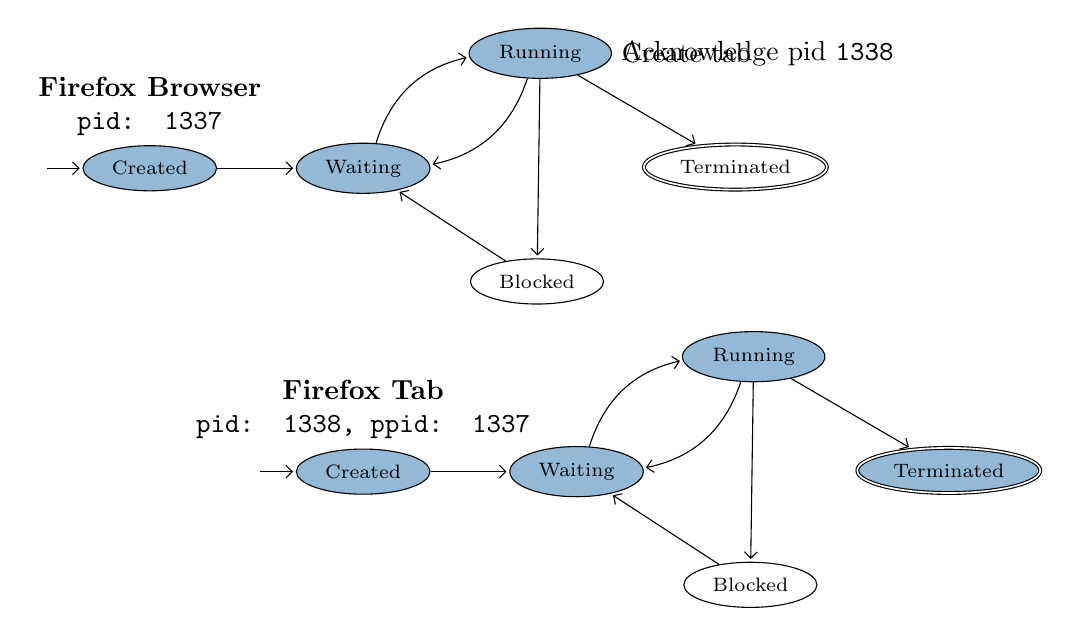
\begin{tikzpicture}[
      every state/.style={ellipse, minimum width=1.25cm, minimum height=0.5cm, font=\scriptsize},
    ]
      \node [state, initial, background fill=uclablue!50,fill on=<1>] (created) {Created};
      \node [state, right=of created, background fill=uclablue!50,fill on=<{2,4-6,8-10,12-14,16-17}>] (waiting) {Waiting};
      \node [state, above right=of waiting, background fill=uclablue!50,fill on=<{3,7,11,15,18}>] (running) {Running};
      \node [state, below right=of waiting] (blocked) {Blocked};
      \node [state, accepting, below right=of running] (terminated) {Terminated};
      \path [->] (created) edge (waiting)
                 (waiting) edge [bend left] (running)
                 (running) edge [bend left] (waiting)
                 (running) edge (blocked)
                 (blocked) edge (waiting)
                 (running) edge (terminated);

      \node <3> [node distance=0, anchor=west, right= of running] {Create tab};
      \node <15> [node distance=0, anchor=west, right= of running] {Acknowledge pid \texttt{1338}};

      \node [align=center, node distance=0, anchor=south, above=of created] {\bfseries Firefox Browser \\ \texttt{pid: 1337}};

      \node <5-16> [state, initial, below left=of blocked, yshift=-1cm, background fill=uclablue!50,fill on=<5>] (created2) {Created};
      \node <5-16> [state, right=of created2, background fill=uclablue!50,fill on=<{6-8,10-12}>] (waiting2) {Waiting};
      \node <5-16> [state, above right=of waiting2, background fill=uclablue!50,fill on=<{9,13}>] (running2) {Running};
      \node <5-16> [state, below right=of waiting2] (blocked2) {Blocked};
      \node <5-16> [state, accepting, below right=of running2, background fill=uclablue!50,fill on=<{14-16}>] (terminated2) {Terminated};
      \path <5-16> [->] (created2) edge (waiting2)
                 (waiting2) edge [bend left] (running2)
                 (running2) edge [bend left] (waiting2)
                 (running2) edge (blocked2)
                 (blocked2) edge (waiting2)
                 (running2) edge (terminated2);

      \node <5-16> [align=center, node distance=0, anchor=south, above=of created2] {\bfseries Firefox Tab \\ \texttt{pid: 1338, ppid: 1337}};

    \end{tikzpicture}
  \end{frame}

  \begin{frame}
    \frametitle{Maintaining the Parent/Child Relationship}

    Previously, we made sure that our parent exited last (by using \texttt{sleep})

    \vspace{2em}

    What happens if the parent process exits first, and no longer exists?
  \end{frame}

  \begin{frame}
    \frametitle{The Parent Process is Responsible for Its Child}

    The operating system sets the exit status when a process terminates
    
    (the process terminates by calling \texttt{exit})

    \hspace{2em} It can't remove its PCB yet

    \vspace{2em}

    The minimum acknowledgment the parent has to do is read the child's exit status

    \vspace{2em}

    There's two situations:
    \begin{enumerate}
      \item The child exits first (zombie process)
      \item The parent exits first (orphan process)
    \end{enumerate}
  \end{frame}

  \begin{frame}
    \frametitle{You Need to Call \texttt{wait} on Child Processes}

    \texttt{wait} as the following API:
    \begin{itemize}
      \item \texttt{status}: Address to store the wait status of the process
      \item Returns the process ID of child process

            \hspace{2em} -1: on failure

            \hspace{2em} 0: for non blocking calls with no child changes

            \hspace{2em} >0: the child with a change
    \end{itemize}

    \vspace{2em}

    The wait status contains a bunch of information, including the exit code

    \hspace{2em} Use \texttt{man wait} to find all the macros to query wait status

    \hspace{4em} You can use \texttt{waitpid} to wait on a specific child process
  \end{frame}

  \begin{frame}[fragile]
    \frametitle{\texttt{wait-example.c} Blocks Until The Child Process Exists, and Cleans Up}

    \begin{lstlisting}
int main(int argc, char *argv[]) {
  pid_t pid = fork();
  if (pid == -1) {
    return errno;
  }
  if (pid == 0) {
    sleep(2);
  }
  else {
    printf("Calling wait\n");
    int wstatus;
    pid_t wait_pid = wait(&wstatus);
    if (WIFEXITED(wstatus)) {
      printf("Wait returned for an exited process! pid: %d, status: %d\n",
             wait_pid, WEXITSTATUS(wstatus));
    }
  }
  return 0;
}
    \end{lstlisting}
  \end{frame}

  \begin{frame}
    \frametitle{A Zombie Process Waits for Its Parent to Read Its Exit Status}

    The process is terminated, but it hasn't been acknowledged

    \vspace{2em}

    A process may have an error in it, where it never reads the child's exit status

    \vspace{2em}

    The operating system can interrupt the parent process to acknowledge the child

    \hspace{2em} It is just a suggestion and the parent is free to ignore it

    \hspace{4em} This is a basic form of IPC called a signal

    \vspace{4em}

    The operating system has to keep a zombie process until it's acknowledged

    \hspace{2em} If the parent ignores it, the zombie process needs to wait to
    be re-parented
  \end{frame}

  \begin{frame}
    \frametitle{An Orphan Process Needs a New Parent}

    The child process lost its parent process

    \hspace{2em} The child still needs a process to acknowledge its exit

    \vspace{2em}

    The operating system re-parents the child process to \texttt{init}

    \hspace{2em} The \texttt{init} process is now responsible to acknowledge the
                 child
  \end{frame}

  \begin{frame}[fragile]
    \frametitle{\texttt{orphan-example.c} The Parent Exits Before the Child, \texttt{init} Cleans Up}

    \begin{lstlisting}
int main(int argc, char *argv[]) {
  pid_t pid = fork();
  if (pid == -1) {
    int err = errno;
    perror("fork failed");
    return err;
  }
  if (pid == 0) {
    printf("Child parent pid: %d\n", getppid());
    sleep(2);
    printf("Child parent pid (after sleep): %d\n", getppid());
  }
  else {
    sleep(1);
  }
  return 0;
}

    \end{lstlisting}
  \end{frame}

  \begin{frame}[fragile]
    \frametitle{\texttt{zombie-example.c} The Parent Monitors the Child To Check Its State}

    \begin{lstlisting}
  pid_t pid = fork();
  // Error checking
  if (pid == 0) {
    sleep(2);
  }
  else {
    // Parent process
    int ret;
    sleep(1);
    printf("Child process state: ");
    ret = print_state(pid);
    if (ret < 0) { return errno; }
    sleep(2);
    printf("Child process state: ");
    ret = print_state(pid);
    if (ret < 0) { return errno; }
  }
    \end{lstlisting}
  \end{frame}

  \begin{frame}
    \frametitle{You're Responsible for Managing Processes}

    The operating system maintains a strict parent/child relationship
    
    \vspace{2em}
    
    You should be able to identify (and prevent) the following:
    \begin{itemize}
      \item Zombie processes
      \item Orphan processes
    \end{itemize}
  \end{frame}
\end{document}
